\chapter{Cook-Levin Theorem}

\section{Cook-Levin Theorem}

\begin{theorem}
    \(SAT\) is NP-complete 
\end{theorem}
\begin{proof}
    There are 2 lemma need to be proved:

    \begin{lemma}[Lemma1: NP]
        \(SAT \in NP\) 
    \end{lemma}
    \begin{proof}
        This is already done
    \end{proof}

    \begin{lemma}[Lemma2: NP-hard]
        If \(\forall A \in NP\), we have \(A \leq_P SAT\).  
    \end{lemma}
    \begin{proof}
        \(A \in NP\): \(A \in NP\) be decided by NTM \(M\) in time \(n^k\).   

        We want to prove there's a polynomial reduction function \(f: \Sigma^* \mapsto formula\) mapping \(A\) to \(SAT\), so:
        \begin{itemize}
            \item \(f(w) = \langle \phi_{M, w} \rangle\)
            \item \(w \in A \iff \phi_{M, w} is satisfiable\)  
        \end{itemize}

        IDEA: the reduction for \(A\) takes a string \(w\) and produces a CNF \(\phi\) that simulates the NP machine for \(A\) on input \(w\).    
        \begin{itemize}
            \item If the machine accepts, \(\phi\) is satisfiable.
            \item If the machine doesn't accept, no assignment satisfies \(\phi\).   
        \end{itemize}

    \end{proof}
    \begin{proof}[Cont.]
        What we do is to transform the problem into a history of \(M\) accepting \(w\):  

        \begin{definition}[tableau]
            An (accepting) tableau for NTM \(M\) on \(w\) is an \(n^k \times n^k\) table representing the computation history for \(M\) on \(w\) on an accepting branch of the nondeterministic computation.     

            \begin{figure}[H]
               \centering 
               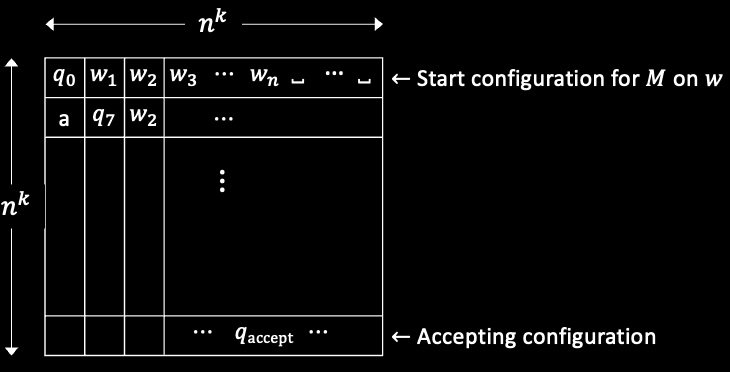
\includegraphics[width=0.8\textwidth]{l16.1.jpg}
               \caption{Example of tableau}
            \end{figure}

            Notice that for NTM, this is only one of the branch which ends up in an accept state.
        \end{definition}

        Now we need to construct \(\phi_{M,w}\)  making it represent that "\(M\) accepts \(w\)",
        which is equal to that a tableau exists for \(M\) on \(w\) exists.   

        The formula \(\phi_{M,w}\) can be represented as following:
        \[
            \phi_{M, w} = 
                \phi_{cell} \land 
                \phi_{start} \land
                \phi_{move} \land
                \phi_{accept}
        \] 
        now we will explain the 4 parts one by one.

        \textbf{1. \( \phi_{cell}\)}: each cell of the tableau can be a state, an alphabet or an empty space, that is to say:

        \textcolor{blue}{In every cell} \textcolor{green}{at least one \(Q \cup \Gamma\)} and \textcolor{red}{at most one}. 

        Let \(C = Q \cup \Gamma\), we have:
        \[
            \phi_{cell} = 
            \textcolor{blue}{\bigwedge_{1 \leq i,j\leq n^k}} (
                \textcolor{green}{\bigvee_{\sigma \in C} x_{i, j, \sigma}} 
                \land
                \textcolor{red}{\bigwedge_{\sigma, \tau \in C\ \sigma \neq \tau} \overline{x_{i,j, \sigma} \land x_{i, j, \tau}}}
                )
        \]

        \textbf{2. \(\phi_{start}\)}: the start configuration should be serialized as \(q_0 w_1 \cdots w_n \cdots \sqcup\):
        \[
            \phi_{start} = 
            x_{1, 1, q_0} \land 
            x_{1, 2, w_1} \land 
            x_{1, 3, w_2} \land
            \cdots \land
            x_{1, n^k, \sqcup}
        \]

        \textbf{3. \(\phi_{accept}\)}: one of the cell is \(q_{accept}\):
        \[
            \phi_{accept} = \bigvee_{1 \leq j \leq n^k}
        \] 

        \textbf{4. \(\phi_{move}\)}: this guarantees that the computation history proceeds legally. 
        This is achieved by recognize all the legal patterns.

        To explain this, I will show some illegal examples:
        \begin{figure}[H]
            \centering 
            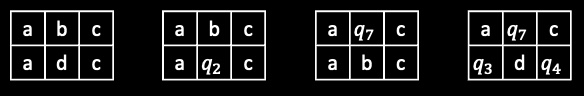
\includegraphics[width=0.8\textwidth]{l16.2.jpg}
            \caption{illegal patterns}
        \end{figure}
    \end{proof}
    \begin{proof}[Cont.]
        And some legal patterns:
        \begin{figure}[H]
            \centering 
            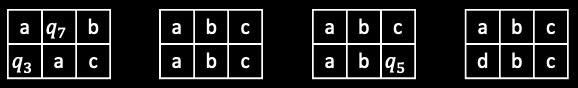
\includegraphics[width=0.8\textwidth]{l16.3.jpg}
            \caption{legal patterns}
        \end{figure}

        So we need to make the window be one of the legal patterns, and this is required by all the windows:
        \[
            \phi_{move} = \bigwedge_{1<i,j<n^k}
            (
                \bigvee_{legal_pattern}
                (
                    x_{i, j-1, r} \land
                    x_{i, j, r} \land
                    x_{i, j+1, r} \land
                    x_{i+1, j-1, r} \land
                    x_{i+1, j, r} \land
                    x_{i+1, j+1, r}
                )
            )
        \]

        The size of \(\phi_{M, w}\) is roughly the size of the tableau for \(M\) on \(w\), so the size is \(O(n^k \times n^k) = O(n^{2k})\)    

    \end{proof}
\end{proof}

\section{SAT3 is NP-complete}
\begin{theorem}
    \(3SAT\) is NP-complete 
\end{theorem}
\begin{proof}
    Because \(SAT\) is NP-complete has already been proved, we just need to prove \(SAT \leq_P 3SAT\) here. 

    A CNF may look like this:
    \[
        \phi = ((a \land b) \lor c) \land (\bar{a} \lor c)
    \]

    The key is first to use transform any conjecture into its result by list all its result:
    
    For \(a \land b\), we can transform it into:
    \[
        ((a \land b) \mapsto z_1) \land 
        ((\bar{a} \land b) \mapsto z_1) \land 
        ((a \land \bar{b}) \mapsto z_1) \land 
        ((\bar{a} \land \bar{b}) \mapsto z_1) \tag{1}
    \] 

    We can transform (1) according to \((A \mapsto B) \mapsto (\bar{A} \lor B)\):
    \[
        (\overline{(a \land b)} \lor z_1) \land 
        (\overline{(\bar{a} \land b)} \lor z_1) \land 
        (\overline{(a \land \bar{b})} \lor z_1) \land 
        (\overline{(\bar{a} \land \bar{b})} \lor z_1) \tag{2}
    \]  

    According to de morgan's law:
    \[
        (a \lor b \lor z_1) \land
        (\bar{a} \lor b \lor z_1) \land
        (a \lor \bar{b} \lor z_1) \land
        (\bar{a} \lor \bar{b} \lor z_1) 
    \]

    This is the same with 3SAT form, and we can do this for all conjectures.
\end{proof}